\documentclass[a4paper,12pt]{article}
\usepackage[utf8]{inputenc}
\usepackage[T1]{fontenc}
\usepackage{graphicx}
\usepackage{longtable}
\usepackage{wrapfig}
\usepackage{rotating}
\usepackage[normalem]{ulem}
\usepackage{amsmath}
\usepackage{amssymb}
\usepackage{capt-of}
\usepackage{hyperref}
\usepackage[margin=20mm]{geometry}
\usepackage{fancyvrb}
\RequirePackage{fancyvrb}

\newcommand\rts[2]{\ensuremath{{#1}_{\text{#2}}}}
\newcommand\bts[2]{\ensuremath{\mathbf{#1}_{\text{#2}}}}

\graphicspath{{./figures}}

\title{Amplifier Control Modes}
\date{\today}

\begin{document}

\maketitle

\section{Electromagnet Model}

\subsection{Governing equations}

Consider one-axis of an eight-pole radial magnetic bearing as shown
below. Here, the number of coil turns per actuator is \(N_c\). to
maintain consistency with existing literature.

\begin{figure}[htbp]
\centering
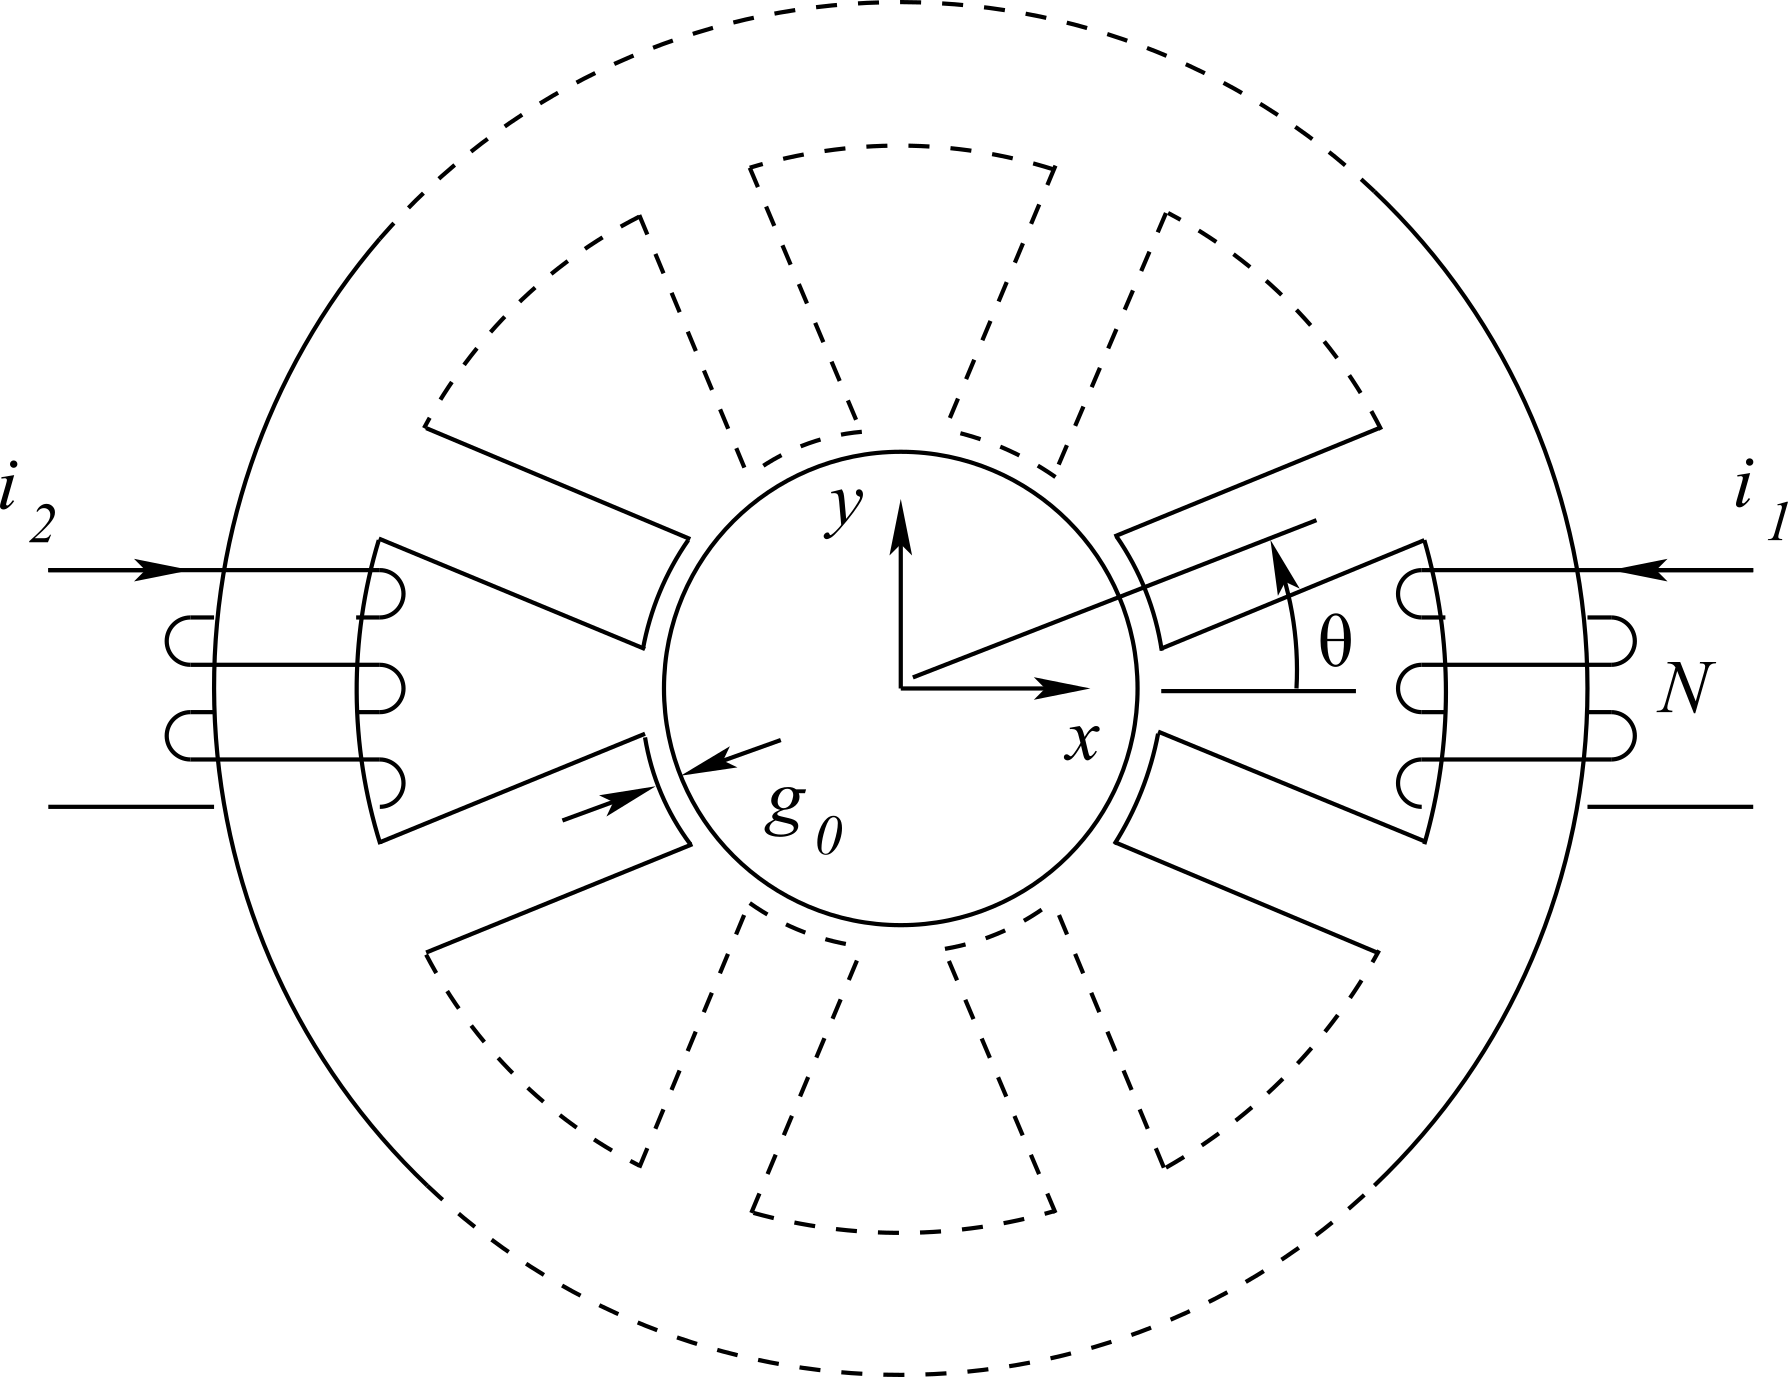
\includegraphics[width=0.5\linewidth]{8p_mag_brg_1dof.png}
\caption{1DOF Actuator}
\end{figure}

Using Maxwell stress tensor, the magnetic force can be expressed as
\begin{equation}
  f_a = \frac{A_p \cos\theta}{\mu_0} ( b_1^2 - b_2^2 )
\end{equation}

Ampere's law
\begin{align}
  \frac{b_1}{\mu_0} \cdot 2(g_0-x\cos\theta) &=  N_c i_1 \\
  \frac{b_2}{\mu_0} \cdot 2(g_0+x\cos\theta) &=  N_c i_2
\end{align}

Faraday's law
\begin{align}
  N_c A_p \dot{b}_1 &= v_1 - R i_1 \\
  N_c A_p \dot{b}_2 &= v_2 - R i_2
\end{align}
Nominal inductance
\[ L_0 = \frac{\mu_0 N_c^2 A_p}{2 g_0} \]

\subsection{Electromagnet Model}

Combining Faraday's law with Ampere's law
\[ N_c A_p \dot{b}_1 = v_1 - R \cdot \frac{2 \left( g_0 - \alpha x
\right)}{\mu_0 N_c} \cdot  b_1 \]
Rearranging this,
\[ \dot{b}_1 = \frac{1}{N_c A_p} v_1 - \frac{R}{L_0} b_1 +
\frac{R}{L_0} \cdot \frac{\alpha x}{g_0} b_1 \]
Similarly,
\[ \dot{b}_2 = \frac{1}{N_c A_p} v_2 - \frac{R}{L_0} b_2 -
\frac{R}{L_0} \cdot \frac{\alpha x}{g_0} b_2 \]

\end{document}
